\chapter[Preliminares ]{Preliminares }\label{ch:capitulo3}

En este capítulo presentaremos diversos términos fundamentales. El objetivo principal es entregar un marco teórico sobre los conceptos que se utilizarán en los siguientes capítulos para definir las técnicas utilizadas.
\begin{definition}[Celdas]
\label{def:cel}
Una celda consiste en una región de la imagen que mide $8$ píxeles de alto por $8$ píxeles de ancho ($8 \times 8$).
\end{definition}

\begin{definition}[Bloques]
\label{def:blo}
Un bloque es una región de la imagen que corresponde a $2 \times 2$ celdas.
\end{definition}

\begin{definition}[Bins]
\label{def:bin}
Un histograma esta compuesto por bins. Un bin es la representación de la cuantificación de un espacio. Generalmente, en el bin se cuenta la cantidad de elementos del espacio que existen en la región definida por dicho bin. 
\end{definition}

\section{Histogram of Oriented Gradients}\label{subsec:hog}
\textit{Histogram of Oriented Gradients} (\textit{HOG}) presentado por Dalal y Triggs~\cite{hog2005}, es un descriptor de características utilizado en visión por computador y procesamiento de imágenes. Este algoritmo sirve para representar objetos (latas, botellas, autos, personas, rostros, etc.). En términos generales, HOG es una técnica que cuenta las ocurrencias de las orientaciones de los gradientes en partes específicas de una imagen. Este método calcula un espacio de celdas superpuestas con el fin de normalizar las muestras locales y aumentar la precisión.

HOG cuenta con ciertos pasos que se deben realizar para obtener el descriptor de una imagen, esto se puede ver en la Figura~\ref{fig:hog_procedure}, y a continuación detallamos las etapas que componen el algoritmo HOG.

\begin{figure}[tb]
  \centering
   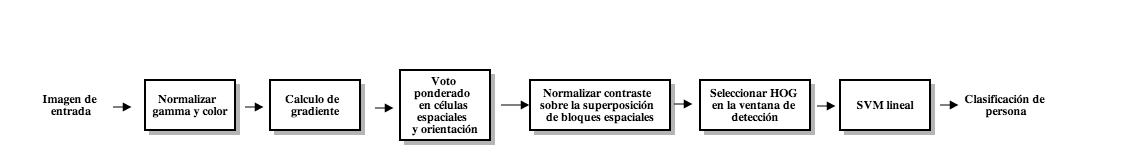
\includegraphics[width=1\textwidth]{Figuras/hog-procedure.png}
   \caption{Procedimiento de cálculo de HOG.}
   \label{fig:hog_procedure}
\end{figure}

\subsection{Procedimiento de HOG}
Felzenszwalb et al.~\cite{Felzenszwalb2010} dividen la imagen en celdas (ver Definición~\ref{def:cel}), sin superposición (en la Figura~\ref{fig:blocks_cells} se puede apreciar la división de los bloques y las celdas antes descritas). Luego, por cada píxel dentro de una celda se acumulan los histogramas de orientación de gradientes. Estos histogramas capturan propiedades de forma local dentro de la celda. a su vez, estos histogramas son invariantes a pequeñas deformaciones.
El gradiente en cada píxel está discretizado en uno de los nueve contenedores (\textit{bins}) de orientación, y cada píxel vota por la orientación de su gradiente, con un valor que depende de la magnitud del gradiente. Para las imágenes en color, se calcula el gradiente de cada canal de color, eligiendo el canal con la mayor cantidad de píxeles donde la magnitud del gradiente esa mayor. 

\begin{figure}[tb]
  \centering
   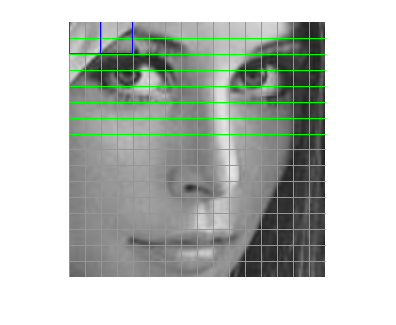
\includegraphics[width=0.5\textwidth]{Figuras/lena-grid.png}
   \caption{Bloque 1 (azul), bloque 2 (rojo), celdas (verde).}
   \label{fig:blocks_cells}
\end{figure}

Finalmente, cada histograma de las celdas es normalizado con respecto a la energía del gradiente en un vecindario alrededor de la celda. Se observan los cuatro bloques de $2 \times 2$ de celdas que contienen una celda particular, y luego se normaliza el histograma cada celda dada con respecto a la energía total en cada uno de estos bloques. Esto entrega un vector de longitud $9 \times 4$ que representa la información local de gradiente dentro de una célula.

\section{Pirámide}\label{sec:pyra}
La pirámide consiste en hacer varias iteraciones de una misma imagen con distintas resoluciones, donde en cada nivel de resolución se extraen las características más representativas con el descriptor de HOG\@. La Figura~\ref{fig:hog_pyra}, muestra los histogramas obtenidos luego de pasar una imagen por tres niveles de la pirámide, estos niveles son representados por $\lambda$ y en la fase de entrenamiento tienen un valor de 5, es decir, cinco niveles de profundidad.

\begin{figure}[tb]
  \centering
   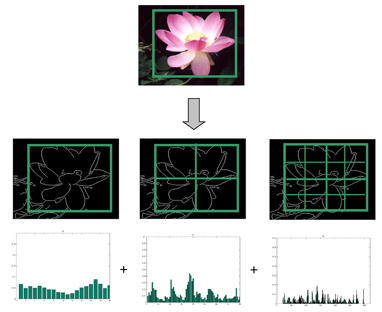
\includegraphics[width=1\textwidth]{Figuras/phog.jpg}
   \caption{Pirámide de HOG~\cite{pyra}}
   \label{fig:hog_pyra}
\end{figure}

\section{Filtro y \textit{score}}\label{sec:fas}

Un filtro está definido por una matriz de $w$ (ancho) por $h$ (alto) la cual define un vector de peso de $d$-dimensiones. Estos filtros especifican las características extraídas por HOG, en los niveles de la pirámide.

El \textit{score} de un filtro está definido por el producto punto entre su vector de pesos y las característica en la sub-ventana de la pirámide de HOG de dimensión $w \times h$.
\section{SVM}\label{sec:lsvm}

\textit{Support Vector Machines} (\textit{SVM})~\cite{Vapnik1995, Duda2000, Cortes1995} es un tipo de algoritmo de aprendizaje supervisado que analiza información y reconoce patrones, utilizado para tareas de clasificación. Dado un conjunto de entrenamiento previamente etiquetado, por ejemplo en dos clases, SVM construye un modelo el cual es capaz de asignar una nueva muestra a una de las categorías previamente definidas, por lo que se define un clasificador binario lineal no-probabilístico.
SVM define un modelo como un conjunto de puntos en un espacio dado que representan un hiper-plano en dicho espacio. Este hiper-plano separa las clases con la mayor diferencia posible para clasificar sin problema dichas clases. Los nuevos datos que entren al modelo serán clasificados en una de las dos opciones de según el lado donde se encuentran respecto al hiper-plano.

Además de realizar la clasificación lineal, SVM puede realizar de manera eficiente una clasificación no lineal utilizando el truco del kernel.% la cartografía de forma implícita sus entradas a los espacios de funciones de alta dimensión. what?!

\subsection{Ventajas de SVM}
\begin{itemize}
\item Eficiente en espacios de dimensiones altas.
\item Sigue siendo eficaz en los casos en que el número de dimensiones es mayor que el número de muestras.
\item Utiliza un subconjunto de puntos de entrenamiento en la función de decisión (llamada vectores de soporte), por lo que también es eficiente en el uso de memoria.
\item Versátil: diferentes funciones del kernel pueden ser especificados para la función de decisión. Kernel comunes se proporcionan, pero también es posible especificar \textit{kernels} personalizados.
\end{itemize}

\subsection{Desventajas de SVM}
\begin{itemize}
\item Si el número de características es mucho mayor que el número de muestras, el método probablemente entregue malos resultados.
\item SVMs no proporcionan directamente las estimaciones de probabilidad.
\end{itemize}

\subsection{Aplicaciones}
\begin{itemize}
\item SVMs es útil en categorización de texto esta aplicación puede reducir significantemente la necesidad de etiquetar instancias del conjunto de entrenamiento.
\item Clasificación de imágenes. 
\item SVMs es útil en la ciencia médica para clasificar las proteínas con hasta un 90\% de los compuestos clasificados correctamente.
\item Reconocimiento de caracteres escritos a mano
\end{itemize}

\section{Resumen}\label{sec:resumen}

Cada uno de los conceptos revisados en este capítulo son de vital importancia para los capítulos posteriores, ya que son estos conceptos los que definirán parte de lo que presentaremos en las siguientes secciones. Esto forma las bases teóricas las cuales darán forma a nuestra propuesta. En nuestro caso es importante destacar el uso de HOG ya que es este algoritmo permite representar de cierta forma las imágenes procesadas, para luego poder clasificarlas con el uso de una variación de SVM, llamada \textit{Latent SVM} (el cual será explicado y detallado en el capítulo siguiente). Términos como \textit{filtro} y \textit{score} serán utilizados con regularidad ya que son estos los que definen porciones importantes del mecanismo de reconocimiento y detección para objetos y expresiones faciales de nuestra propuesta.